\documentclass{handout}


\SetCourseTitle{ECE495: Fundamentals of Robotics Research}
\SetHandoutTitle{Module 2 - Linux for Robotics}
%\SetDueDate{8 Sep at 0715 (via Gradescope)}
%\ShowAllBlanks

%\showsoln \setsolncolor{red}

\newlist{todolist}{itemize}{2}
\setlist[todolist]{label=$\square$}
\usepackage{pifont}
\newcommand{\cmark}{\ding{51}}%
\newcommand{\xmark}{\ding{55}}%
\newcommand{\done}{\rlap{$\square$}{\raisebox{2pt}{\large\hspace{1pt}\cmark}}%
	\hspace{-2.5pt}}
\newcommand{\wontfix}{\rlap{$\square$}{\large\hspace{1pt}\xmark}}

\usepackage{hyperref}

\definecolor{code}{HTML}{ECF8F4}
\definecolor{comments}{HTML}{5269A5}

\usepackage[T1]{fontenc}
\lstset{%
	language=bash, upquote=true,
	otherkeywords={rostopic, rosnode, rosrun, roscore, cd, ls, sudo, nano, echo, mkdir, touch, chmod, catkin\_make, rosmsg, rosservice, catkin\_create\_pkg, rospack, ssh, rosed},
	showspaces=false, showtabs=false, showstringspaces=false, upquote=true, tabsize=4,
	literate={~} {$\sim$}{1},
	showstringspaces=false,
	xleftmargin=0.06\textwidth,
	linewidth=0.99\textwidth,
	columns=fullflexible,
	backgroundcolor=\color{code},
	keepspaces=true,
	breaklines=true,
	basicstyle={\small\fontfamily{fvm}\fontseries{m}\selectfont},
	keywordstyle={\small\fontfamily{fvm}\fontseries{b}\selectfont},
	commentstyle={\color{comments}\small\fontfamily{fvm}\itshape\selectfont},
	belowcaptionskip=10pt,
	float=h
}

\graphicspath{{./figs/}}

\begin{document}
\maketitle

\begin{figure}[H]
	\centering
	
\includegraphics[width=.75\textwidth]{Cover.PNG}
\end{figure}

\textbf{Lesson Objectives:}
\begin{enumerate} \setlength\itemsep{0em}
	\item Learn fundamental concepts of Linux as they apply to robotics.
	\item Develop basic operational understanding of Linux through application.
\end{enumerate}

\textbf{Agenda:}
\begin{enumerate} \setlength\itemsep{0em}
	\item Lecture
	\item ICE2 Jupyter Notebook
\end{enumerate}

\newpage
\clearpage
\pagebreak

\section{Lecture.}
\textbf{Operating System vs Kernel:}
An Operating System is the program that runs on the computer to manage the resources of the system, while the kernel is part of the OS and provides the bridge between the software and hardware.

\textbf{Linux (\url{https://en.wikipedia.org/wiki/Linux}):} "Linux is a family of open source Unix-like operating systems based on the Linux Kernel." Some examples of Linux operating systems include Ubuntu, Debian, Raspbian, Kali, etc. Windows 10 is an operating system and uses Windows-NT as their Kernel. Apple computers use MacOS as their operating system and are based off a Unix Kernel.

A lot of researchers use Linux based operating systems because of the open-source community support.

\soln{1in}{}

\textbf{File Commands:} 
\begin{figure}[H]
	\flushleft
	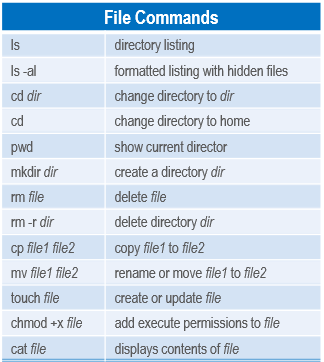
\includegraphics[width=.5\textwidth]{file.PNG}
\end{figure}

\soln{0in}{When working with Windows we often utilize the graphical user interface to navigate the file system. In Linux, we can still use the GUI, but it is often more beneficial to use the command line. This lecture will primarily be used to get you familiar with the command line.}

\textbf{Network/SSH/SCP:} 

\begin{figure}[H]
	\flushleft
	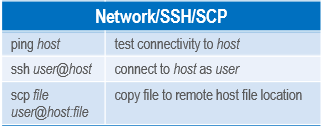
\includegraphics[width=.5\textwidth]{network.PNG}
\end{figure}

\soln{0in}{Linux provides a lot of tools to interact with network interfaces and to remotely communicate with systems. We will be using these tools to work with the robot remotely. Secure shell allows us to run commands from the robot while it is disconnected from a monitor/keyboard/mouse. One command not listed is ifconfig. This is useful to list the current network configurations}

\newpage
\clearpage
\pagebreak

\textbf{Searching:}

\begin{figure}[H]
	\flushleft
	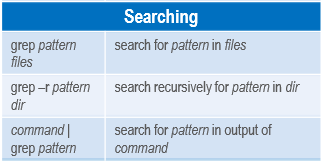
\includegraphics[width=.5\textwidth]{searching.PNG}
\end{figure}

\soln{0in}{Searching for files is sometimes helpful when dealing with complex file systems. These are just some helpeful commands in case you need to search. The last command uses a pipe command which will take one command and pipe it through another command.}

\textbf{Process management:}

\begin{figure}[H]
	\flushleft
	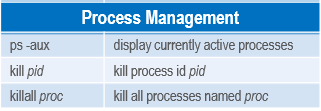
\includegraphics[width=.5\textwidth]{process.PNG}
\end{figure}

\soln{0in}{Process management is sometimes helpful, especially when dealing with ROS to see what programs are running in the background or killing processes that are having issues.}

\textbf{Shortcuts:} 

\begin{figure}[H]
	\flushleft
	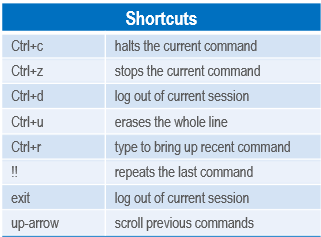
\includegraphics[width=.5\textwidth]{shortcuts.PNG}
\end{figure}

\soln{0in}{These are some usefull shortcuts that help you to be more efficient at command line.} 

\newpage
\clearpage
\pagebreak

\textbf{File permissions:}

\begin{figure}[H]
	\flushleft
	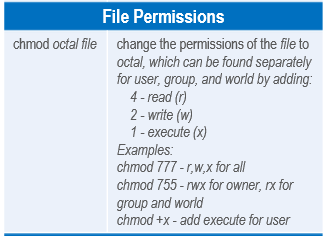
\includegraphics[width=.5\textwidth]{filepermissions.PNG}
\end{figure}

\soln{0in}{File permissions allow yut to set a file to executable.}  

\textbf{System:} 

\begin{figure}[H]
	\flushleft
	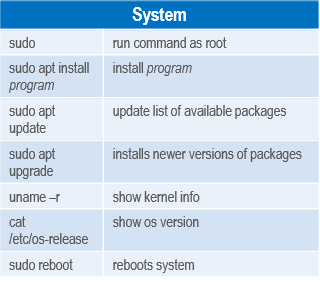
\includegraphics[width=.5\textwidth]{system.PNG}
\end{figure}

\soln{0in}{Just some helpful tools to control the system.}

\section{ICE2 Jupyter Notebook.}
The ICE2 Jupyter Notebook will help you practice implementing some of the discussed Linux commands.

\begin{enumerate}\setlength\itemsep{1em}
	\item On the master, open the Jupyter Notebook server (if it is not already open):
	
\begin{lstlisting}[language=bash]
dfec@master:~$ roscd usafabot_curriculum/Module2_Linux
dfec@master:~$ jupyter-notebook
\end{lstlisting}
	
	\item Open the ICE2 Jupyter Notebook, "ICE2\_Linux.ipynb" and follow the instructions within the notebook. 
\end{enumerate}

\textbf{Checkpoint. Take a screenshot or show the instructor the following:}
\begin{enumerate}
	\item The output of each of the code blocks within the \texttt{ROS} section of the "ICE2\_Linux.ipynb" notebook.
\end{enumerate}

\newpage
\clearpage
\pagebreak

\section{Assignments.}
	\begin{todolist}
		\item Complete Jupyter Notebook if not accomplished during class.
	\end{todolist}

\section{Next time.}
	\begin{itemize}
		\item \textbf{Lesson 5} - Quiz and ICE 2
	\end{itemize}

\end{document}
